\subsection{Approach Overview}


\begin{figure}[t]
	\begin{center}
	  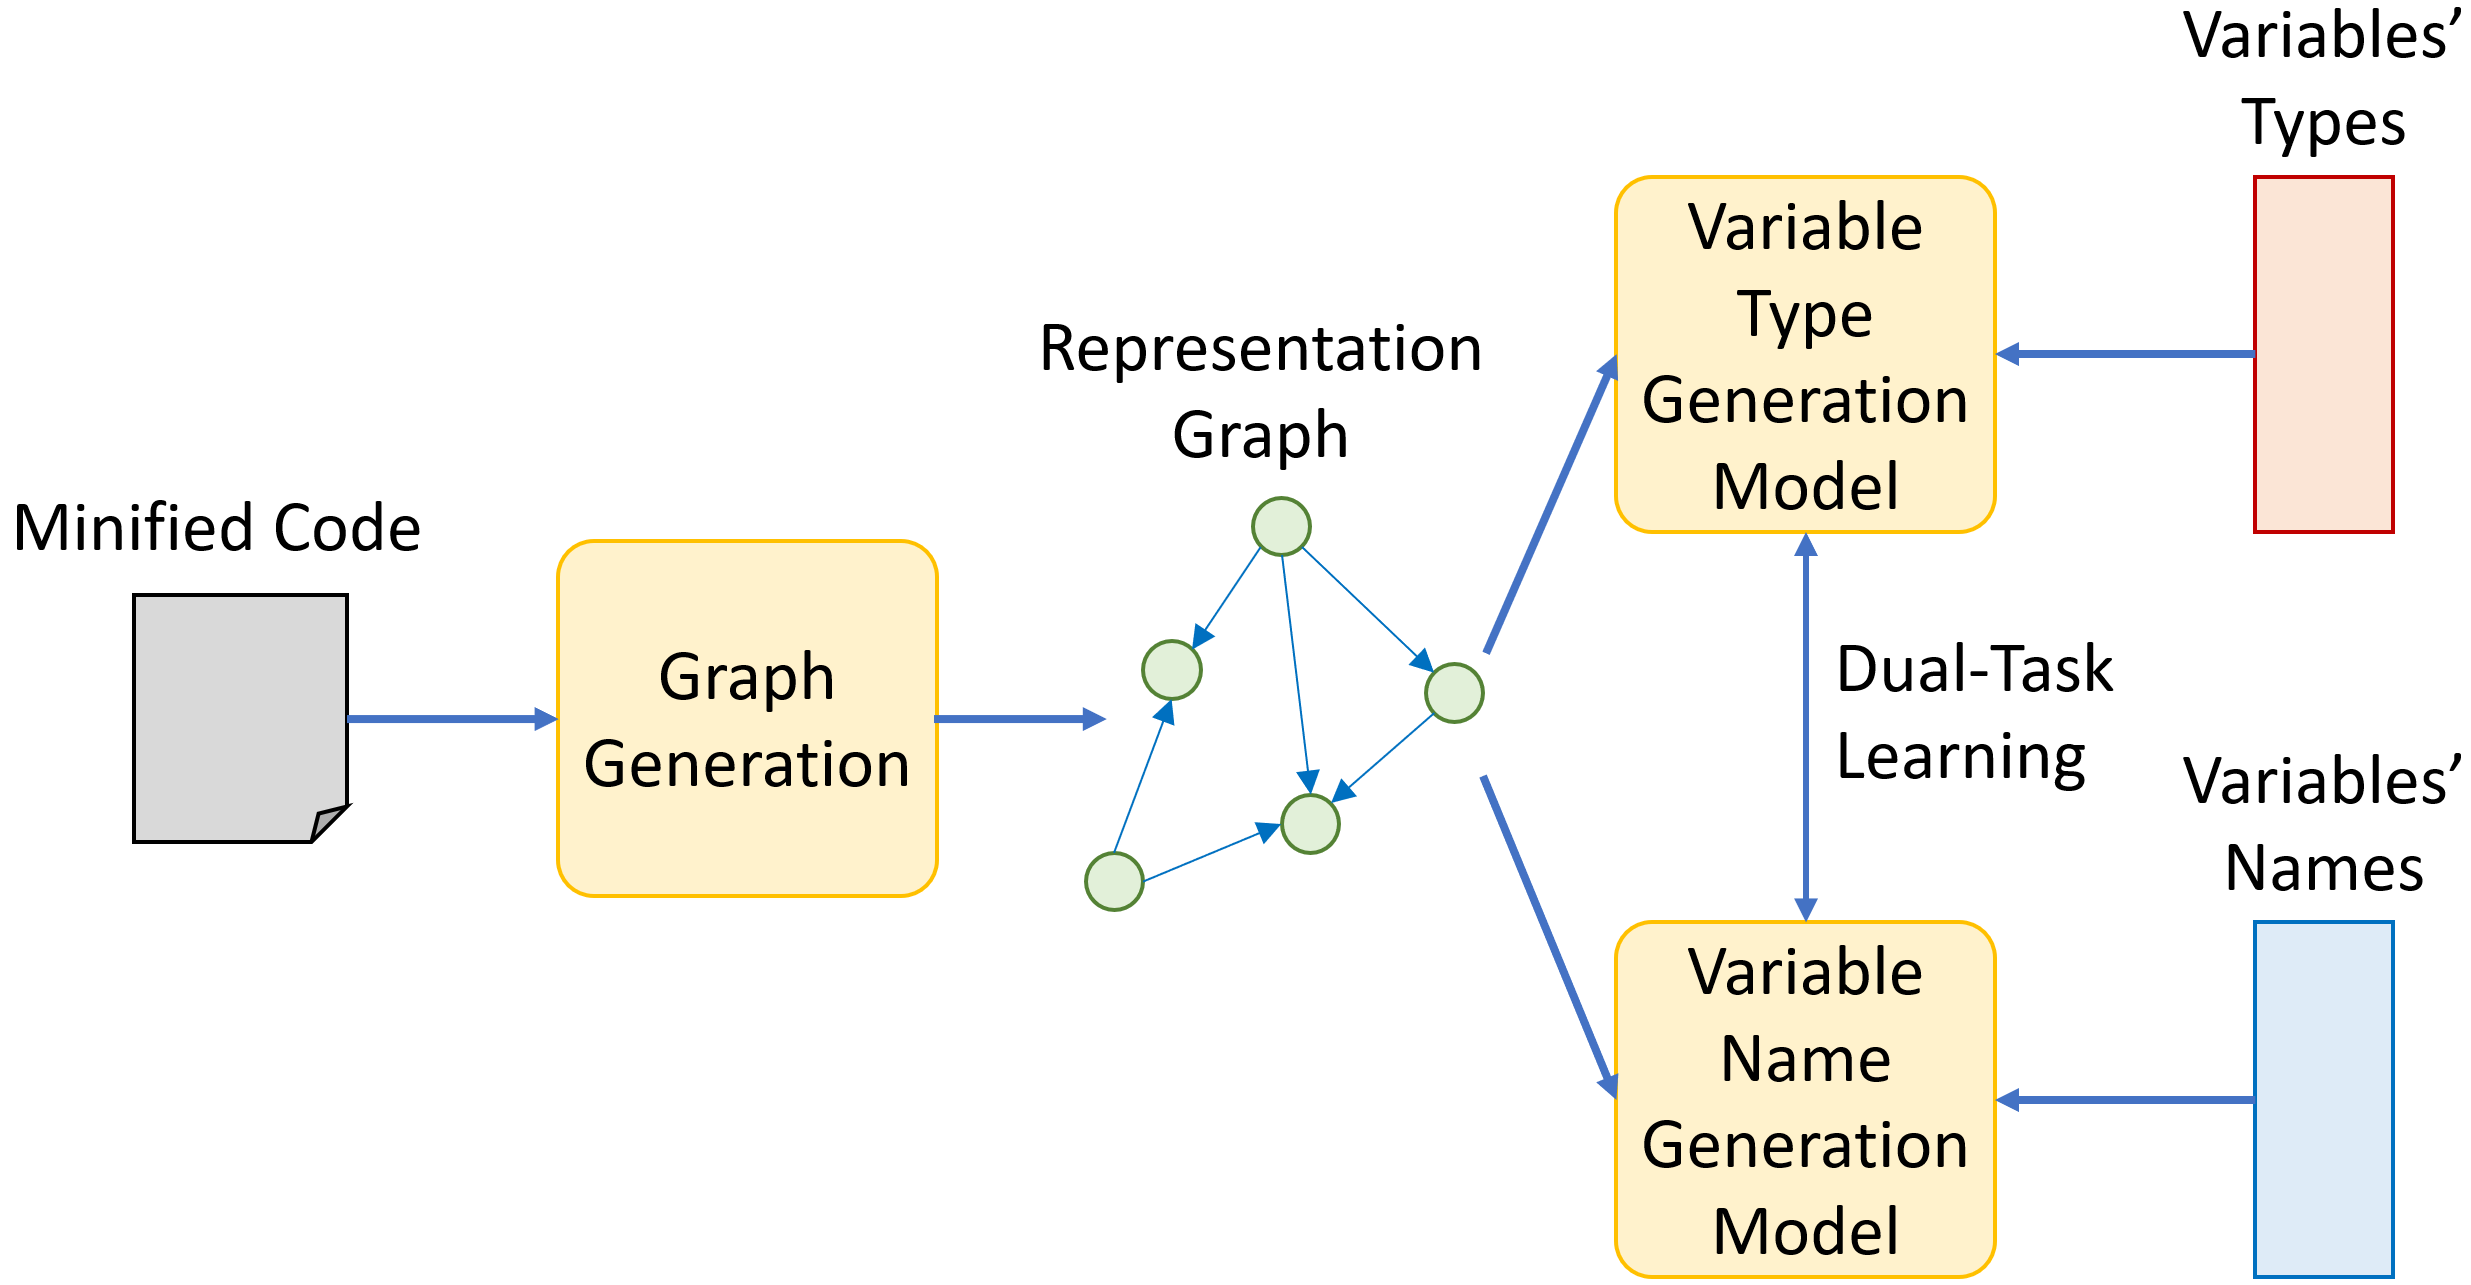
\includegraphics[width=\columnwidth]{figures/training-2.png}
          \vspace{-15pt}
		\caption{Training Process}
		\label{training_process}
	\end{center}
\end{figure}

\begin{figure}[t]
	\begin{center}
		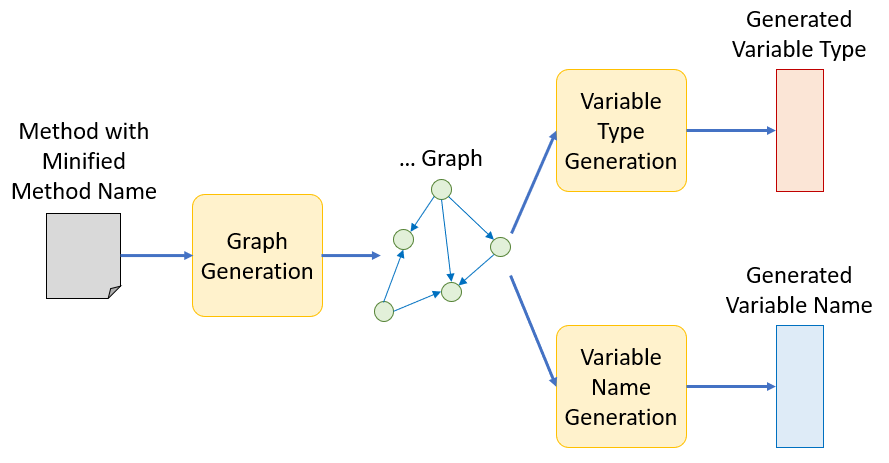
\includegraphics[width=.7\columnwidth]{figures/testing.png}
		\caption{Testing Process}
		\label{testing_process}
	\end{center}
\end{figure}

There are two main processes in {\tool}: training and predicting.

Figure~\ref{training_process} illustrates the training process, which
takes as input the minified code with all the original variables'
names and types. The training process contains the following key
steps. First, we parse the minified code and build two representation
graphs: 1) type relation graph~\cite{} representing the relations
among the types of the variables, and 2) variable relation
graph~\cite{icse19} represent the usage context of a variable with
regard to its field accesses and method calls. The two graphs are
merged into a representation graph.

We have two models dedidated to two tasks: variable type generation
(VTG) and variable name generation (VNG). The VTG model first extracts
the features in a representation graph (e.g., the variables' names,
the names of the fields and methods), and converts them into the input
vectors for the VTG and VNG models. The VTG model leverages a
specialized Graph Convolution Network (GCN)~\cite{} with the support
of the embedding model GloVe~\cite{} as well as the Gate Recurrent
Unit (GRU)~\cite{}. The actual types of the variables in the input
minified code are used as the labels during the training. For type
prediction, the types of the variables are predicted using the trained
VTG model. When generating the types, we use some basic rule from
parser to eliminate the impossible candidates.

The VNG model first extracts the features in the graph and builds the
representation vectors. For the nodes that represent the variables
with the minified names, we mask the node features and regard them as
the missing features, and then feed the graph with missing features
into the a specialized Graph Convolution Network (GCN)~\cite{}. We
leverage that GCN model and others to generate the candidate names for
the minified ones. The actual names of the variables in the input
minified code are used as the labels during the training. For name
prediction, the names of the variables are predicted using the trained
VTG model. When generating the names, we use program analysis rules to
ensure the consistencies among the names.

To propagate the impact of type prediction to name prediction and vice
versa, we apply a dual-task learning mechanism between VTG and VNG
models.  We use the uncertainty weighted multi-task loss as the
multitask learning loss function and use the maximum of the top-1
accuracy score from two tasks as the training target.

%Step 1. Generate graphs...

%Step 2. Variable Type Generation:

%1> Graph edge represent different relations (This may change depends on the graph we finally want to use). Each node is a variable, method call, or a field of an object. We use the name of the variable (minified), method call, or the field as the node feature and use GloVe to learn the representation vector.

%2> We use EGCN that accepts graphs with both node features and edges features as input. Here the edge feature is the edge type. 

%3> The output of EGCN is the generated representation vector $V_r$ for each node. 

%4> We combined the representation vector we get from EGCN with the generated from the next step $V'_r$ (variable name generation) by using the cross-product and get the final generated representation vector for type prediction ($V_f$)

%5> We use a GRU (RNN) as decoder accepts the $V_f$ as input and generates the type for the variables as output.

%6> When generating the type, we use some basic rule from parser to reduce the possible candidates.

%Step 3. Variable Name Generation:

%1> Similar to step 2, we use GloVe to learn the representation vector.

%2> For the node that represent the variable with minified name, we mask the node feature and regard it as the missing feature.

%3> Put the graph with missing feature for some nodes into the $GCN_{mf}$ as input. 

%4> The $GCN_{mf}$ can output the predicted missing node feature representation vector $V_{rm}$ and the node representation vector $V'_r$. The node representation vector $V'_r$ will be used in step 2.

%5> Use $V_{rm}$ as the input of a GRU (RNN) decoder, and the decoder generate the names for the variables with the minified name.

%6> When doing generation, we apply basic checking to make sure the same variable has only one consistent name.

%Step 4. Multi-task learning

%We use the uncertainty weighted multi-task loss as the multitask learning loss function and use the maximum of the top-1 accuracy score from two tasks as the training target.
 
